% =====================================================================================================
% Report del progetto "Multimedia Information Retrieval for Sports Analytics"
% Knowledge graph dei Mondiali FIFA: costruzione, retrieval e valutazione
% Compilare con pdfLaTeX (Overleaf: compilatore pdfLaTeX). Figure in figure/.
% =====================================================================================================
\documentclass[11pt,a4paper]{article}

\usepackage[T1]{fontenc}
\usepackage[utf8]{inputenc}
\usepackage[italian]{babel}
\usepackage{lmodern}
\usepackage{microtype}
\usepackage[a4paper,top=2.3cm,bottom=2.3cm,left=2.4cm,right=2.4cm]{geometry}
\usepackage{graphicx}
\usepackage{booktabs}
\usepackage{tabularx}
\usepackage{array}
\usepackage{multirow}
\usepackage{xcolor}
\usepackage{caption}
\usepackage{pmboxdraw}
\usepackage{rotating}
\usepackage{enumitem}
\usepackage{tikz}
\usetikzlibrary{arrows.meta,positioning,fit,calc}
\usepackage{pgfplots}
\pgfplotsset{compat=1.17}
\usepackage[hidelinks]{hyperref}

\captionsetup{font=small,labelfont=bf}
\setlist{nosep,leftmargin=1.4em}
\setlength{\parskip}{3pt}
\renewcommand{\arraystretch}{1.12}
\newcommand{\code}[1]{\texttt{\small #1}}
\newcolumntype{Y}{>{\raggedright\arraybackslash}X}

\definecolor{dati}{HTML}{5C6670}
\definecolor{grafo}{HTML}{2A57A3}
\definecolor{sem}{HTML}{0D7559}
\definecolor{app}{HTML}{6B4A9E}
\definecolor{valut}{HTML}{A85A16}

\title{\textbf{Un knowledge graph dei Mondiali FIFA\\per il Multimedia Information Retrieval}\\[4pt]
\large Progetto di Multimedia Information Retrieval for Sports Analytics}
\author{Nome Cognome \\ \small Matricola 000000} % TODO: inserire nome, cognome e matricola
\date{Anno accademico 2025/2026}

\begin{document}
\maketitle

\begin{abstract}
\noindent Il progetto costruisce un knowledge graph (KG) dei Mondiali di calcio FIFA a partire da quattro fonti eterogenee: un database relazionale che copre tutti i tornei maschili e femminili dal 1930 al 2022, le classifiche finali dei tornei maschili, le statistiche dei giocatori del Mondiale 2022 e 41.510 immagini dei convocati del 2022. Le fonti vengono pulite e integrate con una procedura di entity resolution, descritte da un'ontologia progettata per il dominio, trasformate in 872.690 triple RDF e caricate in Neo4j (126.744 nodi, 273.516 archi). Sul grafo si interroga con query Cypher che combinano la traversata esatta, un indice full-text sui nomi e due ricerche semantiche: sulle descrizioni dei nodi (MiniLM) e sulle immagini (CLIP). Le domande si pongono con una ricerca guidata oppure in linguaggio naturale, tradotte in Cypher da un modello linguistico (Gemini). La valutazione usa il grafo stesso come risposta di riferimento: unire il filtro del grafo alla ricerca semantica porta l'nDCG@10 da 0,450 a 0,580; CLIP raggiunge una precisione di 0,80 sui concetti visivi; sei domande di analisi su sette non hanno risposta in nessun dataset preso da solo.
\end{abstract}

% =====================================================================================================
\section{Introduzione ai knowledge graph}
% =====================================================================================================

\subsection{Che cos'è un knowledge graph}
Un knowledge graph rappresenta la conoscenza su un dominio come un grafo: i nodi sono entità (un giocatore, una partita, un torneo) e gli archi sono relazioni tra entità (\emph{il giocatore ha segnato nella partita}). Il significato dei tipi di nodo e di arco è fissato da un'\emph{ontologia}, cioè uno schema che definisce classi, proprietà, domini e codomini. Esistono due modelli principali:
\begin{itemize}
  \item il modello \textbf{RDF}, in cui tutta la conoscenza è un insieme di triple \emph{soggetto--predicato--oggetto} identificate da URI, con ontologie scritte in RDFS e OWL e vocabolari condivisi come SKOS. È lo standard del Web semantico e favorisce l'interoperabilità: una risorsa può essere collegata a basi di conoscenza esterne come DBpedia;
  \item il modello a \textbf{grafo con proprietà} (property graph) dei database come Neo4j, in cui nodi e archi hanno etichette e attributi e si interrogano con linguaggi come Cypher.
\end{itemize}
In questo progetto i due modelli lavorano insieme: l'ontologia e le triple RDF fanno da contratto e da formato di scambio, mentre Neo4j fornisce il motore di interrogazione e gli indici di ricerca.

\subsection{Tecniche di costruzione}
Un KG si costruisce da dati non strutturati (estrazione di entità e relazioni dal testo), semi-strutturati o strutturati. Le fonti di questo progetto sono strutturate (tabelle e un database relazionale) più una collezione di immagini; i passi principali sono quindi:
\begin{enumerate}
  \item \textbf{progettazione dello schema}: le classi e le relazioni del dominio, con la fonte di ogni attributo;
  \item \textbf{mappatura} dalle tabelle allo schema: ogni riga diventa un nodo, ogni chiave esterna un arco, ogni colonna una proprietà;
  \item \textbf{entity resolution}: riconoscere la stessa entità in fonti diverse, dove i nomi sono scritti in modi diversi e non c'è un identificativo comune;
  \item \textbf{collegamento} a risorse esterne (\emph{entity linking}), per esempio con \code{owl:sameAs} verso DBpedia, da usare solo quando l'identità è vera;
  \item \textbf{validazione}: controllo delle triple contro l'ontologia e di vincoli di integrità sul grafo finito.
\end{enumerate}

\subsection{Perché un knowledge graph per l'information retrieval}
Un KG porta all'information retrieval quattro vantaggi rispetto a tabelle separate o a una ricerca su testo:
\begin{itemize}
  \item \textbf{integrazione}: fonti diverse diventano un solo grafo, in cui un'informazione che nasce dall'incontro di due fonti (i gol di un giocatore e le scarpe che indossa) si ottiene con una sola query;
  \item \textbf{domande su più passaggi} (multi-hop): \emph{i club dei marcatori nella fase a eliminazione} attraversa partite, fasi, gol, convocazioni e club;
  \item \textbf{risposte esatte e spiegabili}: la query è il percorso che ha prodotto la risposta e si può mostrare all'utente;
  \item \textbf{ricerca ibrida}: la struttura esatta del grafo si combina con la ricerca per somiglianza (embedding di testi e immagini), come nei sistemi di \emph{retrieval-augmented generation} basati su grafi.
\end{itemize}

\subsection{Obiettivi del progetto e task di retrieval}
La traccia chiede un KG sportivo sul Mondiale FIFA 2022, con preprocessing delle fonti, uno schema ontologico, l'estrazione di feature dai dati multimediali, la memorizzazione in un database a grafo, query di retrieval e una valutazione. Il grafo costruito copre \emph{tutti} i Mondiali maschili e femminili dal 1930 al 2022, perché la fonte principale li contiene e le domande storiche danno contesto a quelle sul 2022; il Mondiale 2022 resta il cuore multimediale e statistico, perché immagini, club e statistiche dei giocatori esistono solo per quell'edizione.

Il \textbf{task di retrieval} scelto è il \emph{question answering analitico e multimodale}: rispondere a domande su giocatori, squadre, partite e tornei con schede, classifiche e immagini, anche quando l'entità è descritta senza nome o la domanda riguarda il contenuto di una foto. La Figura~\ref{fig:pipeline} riassume la pipeline; i capitoli seguenti la descrivono in ordine.

\begin{figure}[t]
\centering
\begin{tikzpicture}[
  nodo/.style={draw=#1, fill=#1!8, very thick, rounded corners=2pt, align=center, font=\scriptsize,
               minimum height=1.1cm, text width=2.5cm, inner sep=2pt},
  freccia/.style={-{Latex[length=2mm]}, thick, gray!70!black}]
  \node[nodo=dati] (fonti) {\textbf{4 fonti}\\SQLite, CSV, immagini};
  \node[nodo=dati, right=0.4cm of fonti] (pre) {\textbf{Preprocessing}\\pulizia ed entity resolution};
  \node[nodo=grafo, right=0.4cm of pre] (onto) {\textbf{Ontologia}\\26 classi\\OWL, RDFS, SKOS};
  \node[nodo=grafo, right=0.4cm of onto] (tab) {\textbf{Tabelle integrate}\\una per classe\\(Parquet)};
  \node[nodo=grafo, right=0.4cm of tab] (rdf) {\textbf{Triple RDF}\\872.690 triple\\(rdflib)};
  \node[nodo=grafo, below=0.7cm of rdf] (neo) {\textbf{Neo4j + n10s}\\126.744 nodi\\273.516 archi};
  \node[nodo=sem, left=0.4cm of neo] (ind) {\textbf{Indici}\\full-text, CLIP, MiniLM};
  \node[nodo=app, left=0.4cm of ind] (ret) {\textbf{Retrieval}\\A: ricerca guidata\\B: LLM $\to$ Cypher};
  \node[nodo=app, left=0.4cm of ret] (appn) {\textbf{App}\\Streamlit};
  \node[nodo=valut, left=0.4cm of appn] (val) {\textbf{Valutazione}\\benchmark E2, E3\\grafo vs fonti};
  \draw[freccia] (fonti) -- (pre); \draw[freccia] (pre) -- (onto); \draw[freccia] (onto) -- (tab);
  \draw[freccia] (tab) -- (rdf); \draw[freccia] (rdf) -- (neo); \draw[freccia] (neo) -- (ind);
  \draw[freccia] (ind) -- (ret); \draw[freccia] (ret) -- (appn);
  \draw[freccia] (ret.south) -- ++(0,-0.3) -| (val.south);
\end{tikzpicture}
\caption{Pipeline del progetto. I colori indicano l'area: dati (grigio), grafo (blu), ricerca semantica (verde), interrogazione (viola), valutazione (arancio).}
\label{fig:pipeline}
\end{figure}

% =====================================================================================================
\section{Dati e preprocessing}
% =====================================================================================================

\subsection{Le fonti e le categorie di dati}
La Tabella~\ref{tab:fonti} elenca le quattro fonti. La spina dorsale è il dataset 1, il \emph{Fjelstul World Cup Database}: ha identificativi stabili (\code{P-14758} per un giocatore, \code{M-2022-64} per una partita) e copre tutti i Mondiali con rose, partite ed eventi. Le altre tre fonti aggiungono solo ciò che manca.

\begin{table}[!htb]
\centering\small
\begin{tabularx}{\textwidth}{@{}l l >{\raggedright\arraybackslash}p{3.6cm} Y@{}}
\toprule
\textbf{Dataset} & \textbf{Formato} & \textbf{Dimensione} & \textbf{Cosa aggiunge} \\
\midrule
Dataset 1 & SQLite, 27 tabelle & 30 tornei (22 maschili, 8 femminili), 10.401 giocatori, 1.248 partite & tornei, fasi, gironi, squadre, rose, partite, presenze, gol, cartellini, sostituzioni, rigori, premi, stadi, allenatori, arbitri \\
Dataset 2 & 22 CSV annuali & 489 righe & classifica finale completa dei tornei maschili \\
Dataset 3 & CSV & 814 giocatori del 2022 & club, marca delle scarpe, sponsor tecnico, ranking FIFA, statistiche (assist, dribbling, parate) \\
Dataset 4 & cartelle JPG & 41.510 immagini di 831 giocatori & foto dei convocati 2022 (circa 50 per giocatore), capitano nel nome della cartella \\
\bottomrule
\end{tabularx}
\caption{Le quattro fonti del knowledge graph. Dataset 1: \emph{Fjelstul World Cup Database}; dataset 2: ``FIFA World Cup 1930--2022'' (Sourav Banerjee, Kaggle); dataset 3: ``FIFA WC 2022 Players Stats'' (Rhugved Bhojane, Kaggle); dataset 4: immagini dei giocatori del Mondiale 2022 (Soumendra Prasad, Kaggle).}
\label{tab:fonti}
\end{table}

Le \textbf{categorie di dati} rappresentate sono: struttura dei tornei (torneo, fase, girone, partita, stadio), squadre e organizzazioni (confederazione, federazione, nazionale, partecipazione a un torneo), persone (giocatori, allenatori, arbitri), convocazioni e prestazioni (rosa, presenze, eventi di gioco, premi), dati commerciali del 2022 (club, marche) e contenuti multimediali (immagini).

\subsection{Esplorazione: i problemi trovati}
L'analisi esplorativa ha confrontato ogni fonte con il dataset 1 e ha trovato problemi che, se ignorati, avrebbero prodotto un grafo sbagliato senza messaggi di errore:
\begin{itemize}
  \item \textbf{identità ambigue}: Germania e Germania Ovest hanno lo stesso codice di squadra (\code{DEU}); alcune pagine Wikipedia sono condivise tra una federazione e la sua erede;
  \item \textbf{nomi incoerenti}: 119 partite a gironi non trovano il proprio girone per nome (\emph{group stage} contro \emph{first round}, \emph{Group 1} contro \emph{Group A}, \emph{Group c});
  \item \textbf{nomi corrotti}: 207 nomi di cartella delle immagini erano stati estratti con la codifica sbagliata (\emph{Mbappé} letto come \emph{Mbapp├®});
  \item \textbf{etichette rumorose}: 268 immagini sono duplicate in cartelle di giocatori diversi (lo stesso file compare in 32 cartelle), e 122 file PNG hanno l'estensione \code{.jpg};
  \item \textbf{qualità del dataset 3}: valori mancanti scritti in tre modi diversi, date in quattro formati, refusi nei nomi delle marche, un'emoji nel nome di un giocatore.
\end{itemize}

\subsection{Pulizia}
Ogni fonte è stata pulita senza modificare i file originali. Per il dataset 2 i 22 file annuali sono stati uniti, i nomi delle nazioni allineati al dataset 1 con cinque alias (\emph{USA} $\to$ \emph{United States}) e verificato il sistema dei punti dell'epoca (2 punti per vittoria fino al 1990). Per il dataset 3 sono stati uniformati valori mancanti, tipi e date e corretti i refusi. Per le immagini è stato costruito un indice dei 41.510 file con formato reale e impronta MD5, e i nomi delle cartelle sono stati riparati invertendo l'errore di codifica. I risultati sono salvati in Parquet, che a differenza del CSV conserva i tipi delle colonne (date, interi con valori mancanti).

Un caso istruttivo: dopo l'installazione di \code{pyarrow}, pandas eseguiva le espressioni regolari con il motore RE2, in cui \code{\textbackslash w} comprende solo i caratteri ASCII, e la pulizia cancellava le lettere accentate (\emph{Tchouaméni} $\to$ \emph{Tchouamni}). L'errore è stato scoperto da un controllo sul numero di giocatori abbinati e corretto usando il modulo \code{re} di Python.

\subsection{Entity resolution}
Il dataset 3 e le immagini identificano i giocatori solo per nome, scritto in modo diverso dal dataset 1. L'abbinamento ai \code{player\_id} del dataset 1 procede a cascata e sempre all'interno della stessa nazionale (\emph{blocking}), così si confrontano pochi candidati e si evitano i falsi positivi tra omonimi:
\begin{enumerate}
  \item nome normalizzato identico (traslitterazione, minuscole, solo lettere);
  \item nome simile, con \code{token\_sort\_ratio} di RapidFuzz $\geq 85$;
  \item stessa data di nascita e stesso numero di maglia (solo il dataset 3);
  \item correzione manuale documentata.
\end{enumerate}

\begin{table}[!htb]
\centering\small
\begin{tabular}{@{}l r r r r r@{}}
\toprule
\textbf{Fonte} & \textbf{Nome esatto} & \textbf{Nome simile} & \textbf{Nascita e maglia} & \textbf{Manuale} & \textbf{Non abbinati} \\
\midrule
Dataset 3 (814 righe) & 766 & 28 & 19 & 1 & 0 \\
Dataset 4 (831 cartelle) & 821 & 8 & -- & 1 & 1 \\
\bottomrule
\end{tabular}
\caption{Esito dell'entity resolution. L'unica cartella non abbinata è di un giocatore assente dal dataset 1 (convocato e poi escluso dalla rosa).}
\label{tab:er}
\end{table}

La riparazione dei nomi è un prerequisito: senza di essa gli abbinamenti esatti delle cartelle scendevano da 821 a circa 770.

\subsection{Lo schema ontologico}
L'ontologia (Figura~\ref{fig:ontologia}) ha 26 classi, 26 proprietà oggetto e 67 proprietà dato, per 943 triple OWL, RDFS e SKOS. È generata da un'unica specifica in Python, da cui derivano sia il file Turtle sia la figura. I principi di progettazione sono:
\begin{itemize}
  \item \textbf{una fonte autorevole per ogni attributo}: identità, maglia, ruolo, presenze e gol vengono dal dataset 1; il dataset 3 fornisce solo ciò che il dataset 1 non ha;
  \item \textbf{fatti primari, non totali}: vittorie, punti e gol totali non si importano ma si ricalcolano con le query; i totali delle fonti diventano controlli di coerenza;
  \item \textbf{reificazione solo quando serve}: in RDF un arco non ha attributi, quindi una relazione diventa un nodo solo se ha proprietà proprie o se altri nodi devono puntarla. \emph{Participation} (una squadra in un torneo) è il perno del grafo: ha attributi (ospitante, posizione finale, ranking) e la puntano partite, convocazioni ed eventi, e da lei partono gli archi verso nazionale, torneo e allenatori. Lo stesso vale per \emph{SquadMembership}, \emph{Appearance} e \emph{GroupStanding};
  \item \textbf{gli attributi che cambiano nel tempo stanno sulla convocazione}: maglia, ruolo, capitano, club e premi sono proprietà di \emph{SquadMembership}, non di \emph{Player};
  \item \textbf{riuso di vocabolari standard} (schema.org, FOAF, SKOS) e annotazione della fonte di ogni classe e proprietà.
\end{itemize}

\begin{sidewaysfigure}
\centering
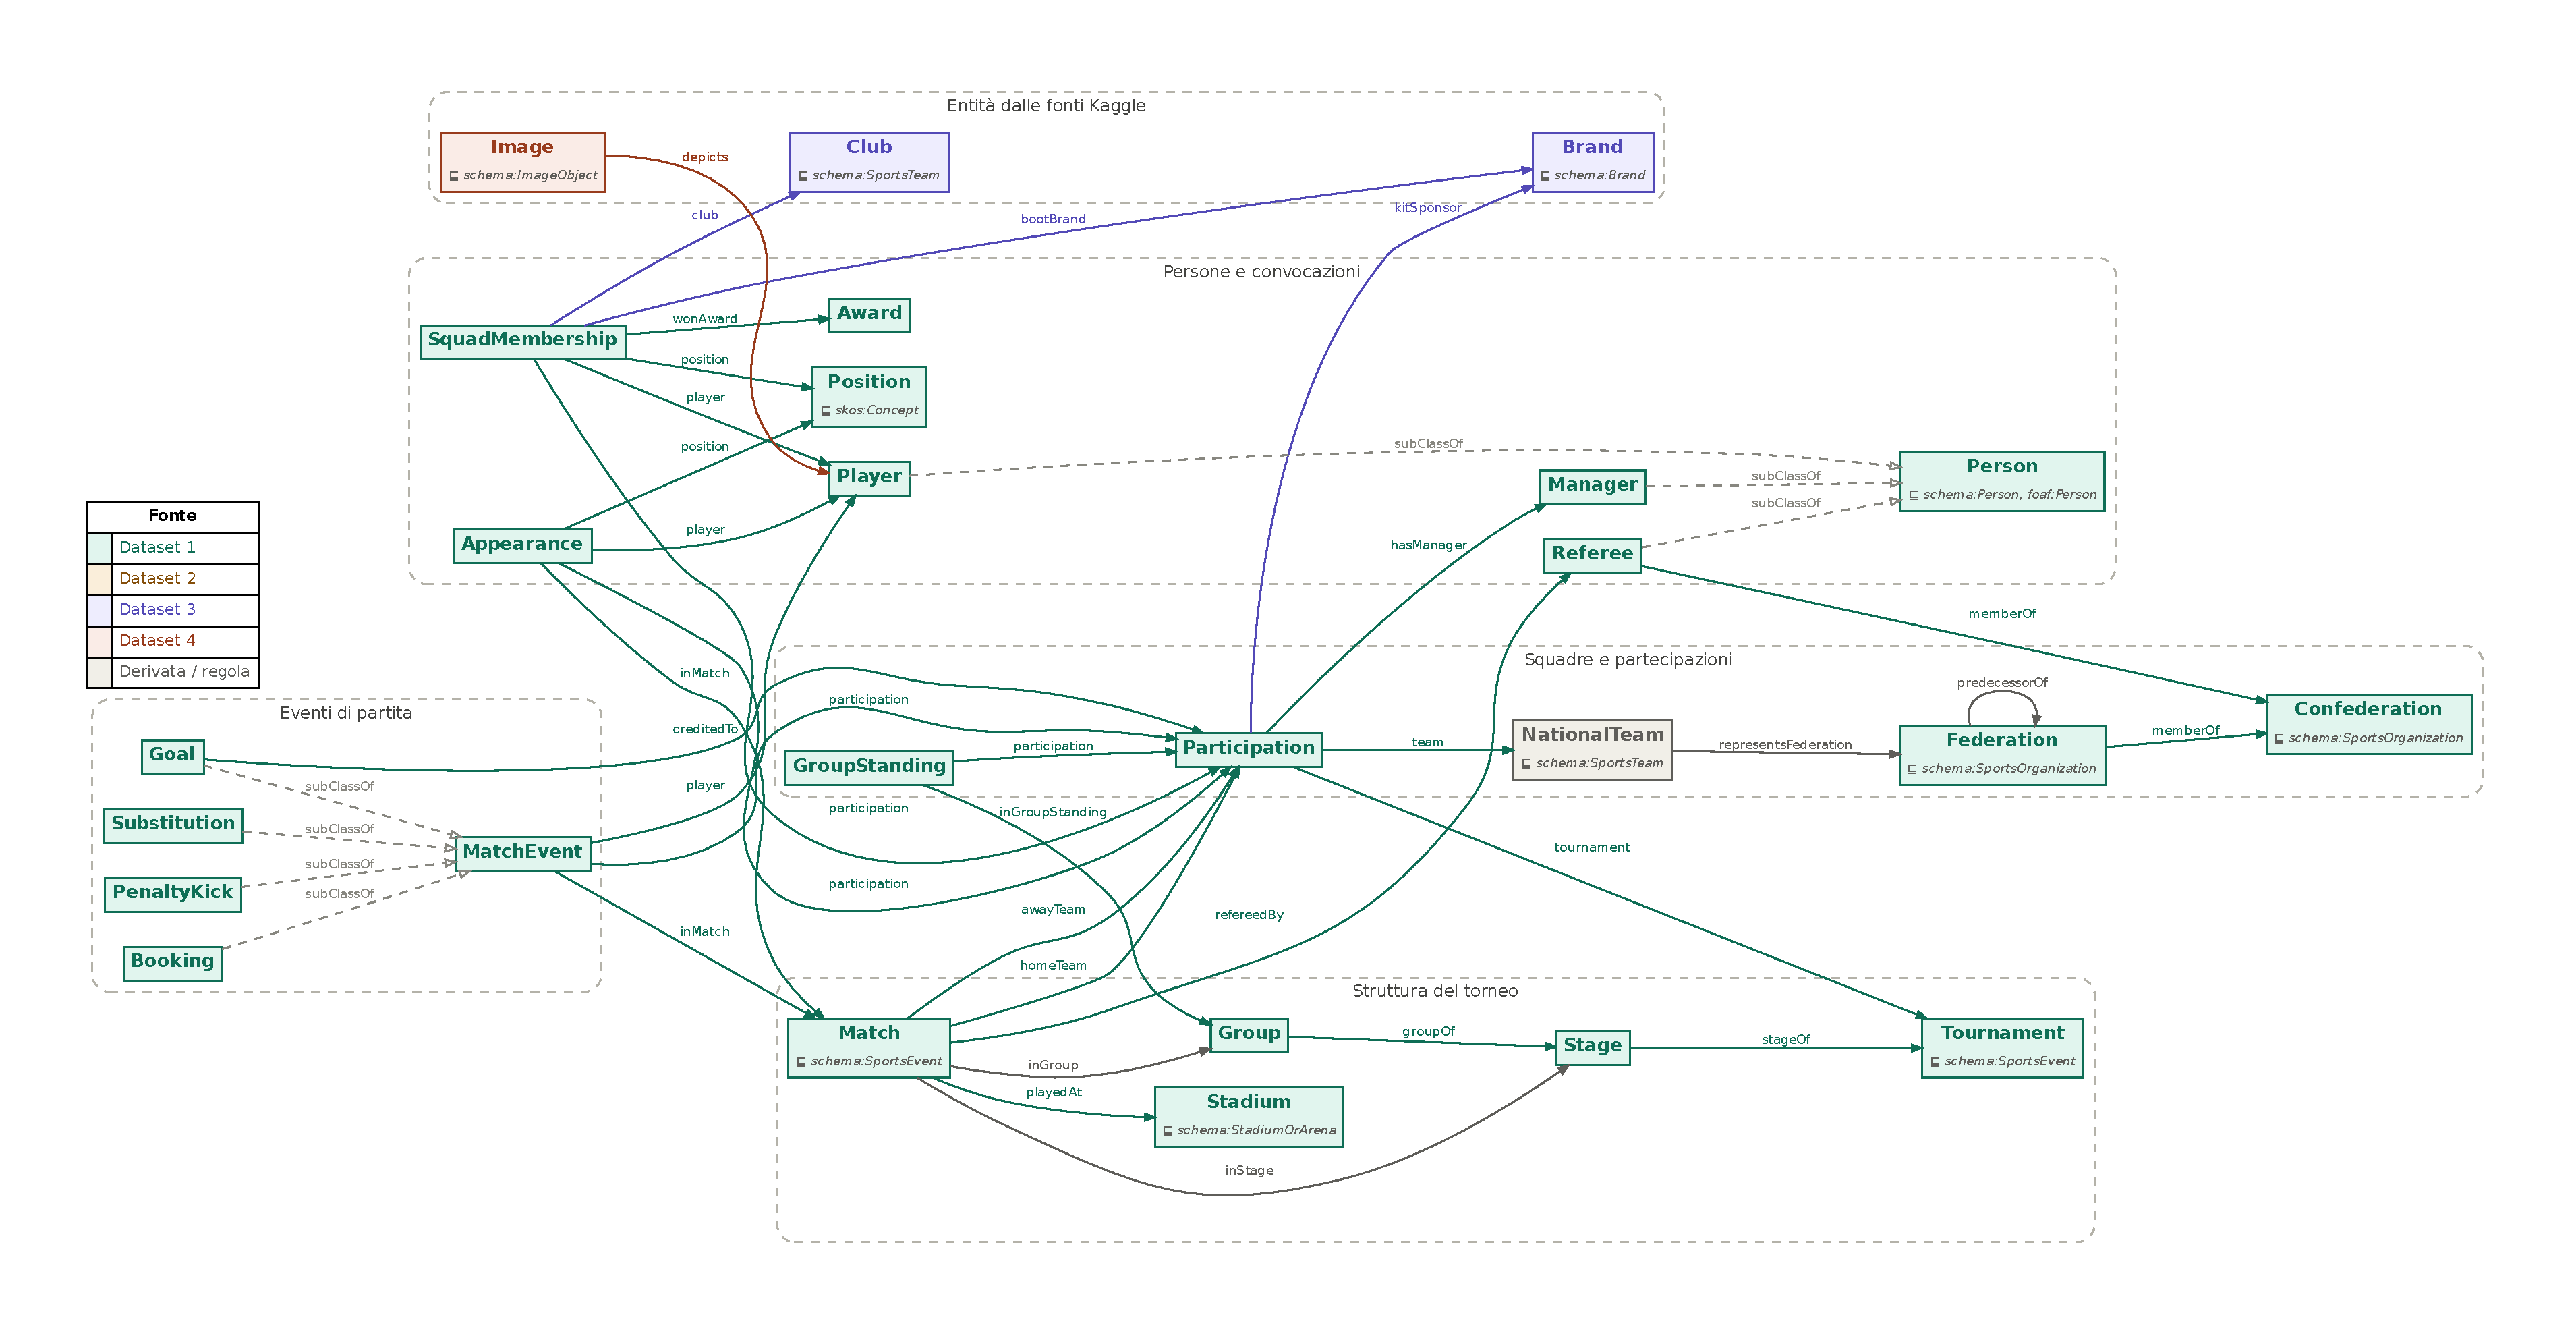
\includegraphics[width=\textheight,height=0.9\textwidth,keepaspectratio]{figure/schema_core.pdf}
\caption{Schema dell'ontologia: classi, relazioni e fonte di ogni elemento (generato da \code{spec.py} con Graphviz). \emph{Participation} collega squadre, tornei, partite, allenatori e convocazioni.}
\label{fig:ontologia}
\end{sidewaysfigure}

Due decisioni mostrano il tipo di problemi risolti dallo schema. \textbf{Partite e gironi}: dato che i nomi dei gironi sono incoerenti, il girone di una partita si ricava dalle due squadre (il girone che, nello stesso torneo, le contiene entrambe); la regola collega 922 partite su 922 a esattamente un girone. \textbf{Identità}: \code{owl:sameAs} è simmetrico e transitivo, quindi usarlo per la Germania Ovest verso la pagina DBpedia della Germania renderebbe le due federazioni la stessa entità; si usa \code{owl:sameAs} solo per l'erede e \code{rdfs:seeAlso} per il predecessore, e la continuità storica è una relazione esplicita (\code{predecessorOf}). La storia secondo la FIFA, con i quattro titoli della Germania, si ricostruisce seguendo quella relazione senza fondere le entità.

% =====================================================================================================
\section{Metodologie di retrieval}
% =====================================================================================================

\subsection{Query strutturate sul grafo}
La forma più diretta di retrieval su un KG è una query nel linguaggio del database: SPARQL per i triple store, Cypher per Neo4j. Una query esatta è precisa e spiegabile, ma richiede di conoscere lo schema e i valori esatti (\emph{Golden Ball}, \emph{PSG}, il ruolo \emph{MF}); un valore scritto in modo diverso dà zero risultati. Per le domande ricorrenti si possono preparare \emph{modelli di query} con parametri, che l'utente riempie con una ricerca guidata.

\subsection{Ricerca lessicale sui nomi}
Per trovare un'entità dal nome si usa un indice full-text (Lucene, integrato in Neo4j), con un punteggio di tipo BM25 e la ricerca \emph{fuzzy}, che tollera qualche lettera sbagliata (\emph{Mbape} $\to$ \emph{Mbappé}). Un analizzatore che toglie accenti e maiuscole rende la ricerca indifferente a come si scrive il nome. La ricerca lessicale è precisa sui nomi propri ma non capisce le parafrasi.

\subsection{Ricerca semantica con embedding}
Un \emph{embedding} è un vettore che rappresenta il significato di un testo o di un'immagine: contenuti simili hanno vettori vicini, misurati con la similarità coseno.
\begin{itemize}
  \item Per il \textbf{testo} si usano modelli di frasi come Sentence-BERT; in questo progetto \code{all-MiniLM-L6-v2}, un modello piccolo (384 dimensioni) ottenuto per distillazione.
  \item Per le \textbf{immagini} si usa CLIP, addestrato su coppie immagine--didascalia: testi e immagini finiscono nello stesso spazio (512 dimensioni), quindi una frase come \emph{a goalkeeper diving} recupera le foto corrispondenti. CLIP è il modo con cui il progetto \emph{estrae feature dai dati multimediali}.
  \item La ricerca dei vettori più vicini usa indici approssimati come HNSW, disponibili in Neo4j accanto al grafo.
\end{itemize}
Un KG ha però pochi testi: per cercare i nodi per significato bisogna prima \emph{verbalizzarli}, cioè scrivere per ogni nodo una frase con i suoi fatti principali, e calcolarne l'embedding.

\subsection{Strategie ibride}
Molte domande uniscono una parte descrittiva e vincoli esatti: \emph{portieri brasiliani al Mondiale 2002}. Esistono due modi di combinare ricerca semantica e grafo nella stessa query:
\begin{itemize}
  \item \textbf{indice prima}: l'indice vettoriale restituisce i $k$ nodi più vicini su tutto il grafo, poi i filtri del grafo li restringono. È veloce, ma se i filtri sono selettivi può scartare tutti i candidati, perché in Neo4j 5.26 il filtro avviene dopo i primi $k$;
  \item \textbf{grafo prima}: la query restringe i nodi con i vincoli esatti e poi calcola la similarità coseno esatta solo su quelli. Non perde risultati e costa poco quando il grafo restringe molto.
\end{itemize}

\subsection{Il ruolo dei modelli linguistici}
I grandi modelli linguistici (LLM) aggiungono due capacità al retrieval su KG: tradurre una domanda in linguaggio naturale in una query (\emph{text-to-Cypher}) e generare risposte a partire dai fatti recuperati (\emph{GraphRAG}). Il primo uso permette domande che nessun modello di query aveva previsto; il rischio è una query sbagliata o, se l'LLM scrive la risposta, un testo inventato. In questo progetto l'LLM scrive solo la query, che viene eseguita in sola lettura e mostrata all'utente; la risposta è sempre il risultato della query.

\subsection{Il valore aggiunto della ricerca semantica}
Se il grafo può già rispondere con una query esatta, la ricerca semantica serve? Il grafo da solo basta quando valgono tre condizioni: ciò che si chiede è salvato come dato, chi scrive la query conosce i valori esatti, e il concetto è preciso. La ricerca semantica serve quando almeno una di queste non vale:
\begin{enumerate}
  \item \textbf{il dato non esiste nel grafo}: il contenuto delle foto (\emph{esulta}, \emph{in tuffo}) esiste solo nei vettori CLIP. È il caso in cui la ricerca semantica è insostituibile;
  \item \textbf{le parole non coincidono con i valori}: \emph{award for the best goalkeeper} contro \emph{Golden Glove}. Una query con il valore sbagliato dà zero righe, la ricerca semantica peggiora gradualmente;
  \item \textbf{la domanda chiede una somiglianza}: \emph{giocatori simili a Modrić} non ha un equivalente Cypher;
  \item \textbf{la query esatta è possibile ma molto complicata}: \emph{finali con una tripletta} richiede di contare i gol per giocatore e partita, mentre la descrizione della partita lo dice già.
\end{enumerate}
Poiché le descrizioni dei nodi sono generate dal grafo, la ricerca su di esse non aggiunge fatti nuovi: aggiunge tolleranza alle parole e somiglianza. Questa distinzione guida la valutazione del Capitolo~\ref{sec:impl}.

% =====================================================================================================
\section{Implementazione del sistema e valutazione}\label{sec:impl}
% =====================================================================================================

\subsection{Costruzione e popolamento del grafo}
La costruzione segue tre passi, ciascuno verificato prima del successivo.
\begin{enumerate}
  \item \textbf{Tabelle integrate.} Per ogni classe dell'ontologia si costruisce una tabella (una riga per istanza, una colonna per proprietà) e, per le relazioni molti-a-molti, tabelle di soli archi. Ogni unione tra fonti è vincolata a essere uno-a-uno, così un'unione sbagliata si ferma subito. Qui si applicano le regole più delicate: il girone delle partite, l'unificazione dei nomi dei club (316 grafie nel dataset 3 diventano 291 club, con 13 alias decisi a mano e 19 coppie simili tenute distinte) e le proprietà del 2022 sulle convocazioni.
  \item \textbf{Triple RDF.} Con \code{rdflib}, una tabella di corrispondenza indica per ogni tabella la classe, il modello dell'URI (per esempio \code{player/\{player\_id\}}), le colonne e gli archi. Gli URI si calcolano dagli identificativi, quindi ogni file si genera da solo e i file si collegano per URI. Il tipo di ogni valore si legge dal codominio dichiarato nell'ontologia, e per i valori mancanti non si scrive nessuna tripla (ipotesi di mondo aperto: l'assenza significa ``non si sa'', non ``falso''). Risultato: 27 file Turtle, 872.690 triple, nessuna violazione di dominio, codominio o tipo.
  \item \textbf{Import in Neo4j.} Le triple entrano in Neo4j 5.26 con il plugin \emph{neosemantics} (n10s), con un vincolo di unicità sull'URI (un solo nodo per URI) e nomi brevi per le proprietà. Il grafo finale ha \textbf{126.744 nodi} in 24 classi e \textbf{273.516 archi} di 27 tipi, più 11.574 risorse esterne (DBpedia e Wikipedia).
\end{enumerate}
Un notebook di verifica in sola lettura ha confermato che il grafo è conforme all'ontologia (51 combinazioni classe--relazione--classe su 51), rispetta 18 vincoli di integrità (per esempio, i gol ricostruiscono il risultato di tutte le 1.248 partite) ed è un'unica componente connessa. Una prova indipendente: gli ospitanti campioni ricavati dal grafo coincidono con una colonna del dataset 1 che non era stata importata.

\subsection{Feature multimediali e descrizioni dei nodi}
\textbf{Immagini.} Per tutte le 41.460 immagini collegate a un giocatore si calcola l'embedding CLIP (ViT-B/32). Dagli embedding si ricava una feature di qualità, \code{labelConfidence}: la similarità coseno tra un'immagine e il centro delle \emph{altre} foto dello stesso giocatore. Un'etichetta sbagliata dà un valore basso; la verifica sulle immagini duplicate tra giocatori diversi, sbagliate almeno per uno dei due, dà un'AUC di 0,745 (media 0,812 per le non duplicate contro 0,732). La scheda di un giocatore mostra l'immagine non duplicata con la confidenza più alta.

\textbf{Descrizioni.} Per i 12.893 nodi di sei classi (giocatori, partecipazioni, partite, federazioni, club, stadi) una frase-modello in inglese riassume i fatti del grafo, per esempio \emph{``Luka Modrić, midfielder for Croatia \dots{} Golden Ball 2018''}; la frase diventa un vettore MiniLM. Le frasi sono state verificate confrontandone dodici con quelle attese, carattere per carattere.

\textbf{Indici.} Sei indici full-text sui nomi e sette indici vettoriali (uno per le immagini, uno per classe descritta). Con la compressione dei vettori attiva per default, l'indice delle immagini aveva in comune con il calcolo esatto solo da 0 a 2 risultati su 5, perché i punteggi CLIP sono molto vicini tra loro; disattivando la compressione e chiedendo 100 candidati per tenere i primi $k$, la concordanza è salita a 5 su 5.

\subsection{Architettura del sistema di retrieval}
Il codice è un pacchetto Python condiviso da notebook, app e valutazione: connessione in sola lettura, ricerca (full-text e vettoriale), modelli di query, descrizioni ed embedding, modulo LLM. La Figura~\ref{fig:architettura} mostra come una domanda diventa una risposta.

\begin{figure}[t]
\centering
\begin{tikzpicture}[
  b/.style={draw=#1, fill=#1!8, very thick, rounded corners=2pt, align=center, font=\footnotesize, inner sep=4pt},
  f/.style={-{Latex[length=2mm]}, thick, gray!70!black}]
  \node[b=app, text width=3.1cm] (bb) {\textbf{B. Domanda libera}\\Gemini riceve schema e regole\\e restituisce un JSON};
  \node[b=app, text width=3.1cm, below=0.5cm of bb] (a) {\textbf{A. Ricerca guidata}\\tipo di domanda e campi\\con suggerimenti};
  \coordinate (m) at ($(a.east)!0.5!(bb.east)$);
  \node[b=sem, text width=3.6cm, right=0.9cm of m] (par) {\textbf{Parametri}\\nomi $\to$ query Lucene\\testi $\to$ vettori MiniLM o CLIP};
  \node[b=grafo, text width=4.0cm, right=0.9cm of par] (q) {\textbf{Query Cypher in sola lettura}\\traversata del grafo\\+ \code{db.index.fulltext}\\+ \code{db.index.vector} / coseno};
  \node[b=dati, text width=4.0cm, below=0.55cm of q] (r) {\textbf{Risposta}\\scheda, tabella, grafico,\\immagini + query eseguite};
  \draw[f] (a.east) -- (par); \draw[f] (bb.east) -- (par); \draw[f] (par) -- (q); \draw[f] (q) -- (r);
  \draw[f, dashed] (q.north) |- node[pos=0.75, above, font=\scriptsize]{errore o risultato vuoto: un nuovo tentativo} ($(bb.north)+(0,0.4)$) -- (bb.north);
\end{tikzpicture}
\caption{Dalla domanda alla risposta. In A i parametri vengono dai campi del modulo; in B dal JSON prodotto da Gemini (\code{cypher}, \code{nomi}, \code{vettori}).}
\label{fig:architettura}
\end{figure}

\textbf{Meccanismo A, ricerca guidata.} L'utente sceglie il tipo di domanda (scheda di un giocatore, di una squadra in un torneo, di una partita, di un torneo, classifica per metrica, testa a testa, entità descritta senza nome, immagini da testo) e riempie i campi; i nomi hanno suggerimenti dall'indice full-text. Ogni tipo ha un modello di query parametrico, controllato su 46 risultati noti (46 su 46 corretti).

\textbf{Meccanismo B, domanda libera.} Una prima versione riconosceva il tipo di domanda per somiglianza con 79 domande di esempio, ma classificava correttamente solo 34 esempi su 79: un embedding di frase riflette l'argomento più dell'intenzione. È stata sostituita da un LLM (Gemini) che riceve lo schema del grafo e alcune regole (nome proprio $\to$ indice full-text; descrizione o contenuto di una foto $\to$ vettore; fatto esatto $\to$ \code{MATCH}/\code{WHERE}) e risponde con un JSON vincolato da uno schema: la query, i nomi da cercare e i testi da trasformare in vettori. L'LLM non vede i dati; la query gira in una transazione di sola lettura e, in caso di errore o risultato vuoto, l'LLM riceve il problema e riprova una volta. Su nove domande di prova, otto hanno dato un risultato; l'errore tipico è un nome ``come dovrebbe essere'' invece che come è nel grafo (\emph{Paris Saint-Germain} contro \emph{PSG}). Per esempio, \emph{a Dutch winger who reached the final in 2010} diventa una query che trova l'Olanda con il full-text, restringe ai convocati della finale 2010 e ordina per similarità con \emph{winger}.

\textbf{App.} Un'app Streamlit espone i due meccanismi e mostra, per ogni risposta, tutte le query Cypher eseguite con i loro parametri.

\subsection{Benchmark e metriche}
La valutazione misura il retrieval a partire dalla query Cypher, lasciando fuori l'LLM, la cui valutazione richiederebbe un protocollo a parte (risposte non deterministiche). L'idea centrale è usare il \textbf{grafo come risposta di riferimento}: per molte domande descrittive esiste una query esatta che calcola l'insieme dei nodi pertinenti, e si misura quanti di questi la ricerca semantica mette in cima. Dove il grafo non può conoscere la risposta (contenuto delle foto, concetti vaghi, somiglianza) la pertinenza è giudicata a mano con un criterio scritto prima di vedere i risultati. Le metriche sono precisione (P@$k$), richiamo (R@10), nDCG@10 e MRR.
\begin{itemize}
  \item \textbf{E2, descrizioni dei nodi}: 21 domande con risposta esatta (dimensioni dell'insieme pertinente da 1 a 22) e 3 giudicate a mano. Le domande usano parole diverse dalle frasi-modello (\emph{Brazilian} invece di \emph{for Brazil}), per non rendere la ricerca perfetta per costruzione. Per ogni domanda i vincoli sono divisi in anticipo tra grafo (anno, fase, ospitante) e semantica (parte descrittiva). Si confrontano: \emph{solo semantica} (domanda intera, nessun filtro), \emph{indice prima} con 50, 100 e 500 candidati, \emph{grafo prima}, e un \emph{controllo}: grafo prima con la domanda intera.
  \item \textbf{E3, immagini (CLIP)}: (a) riconoscimento della persona (\emph{a photo of} + nome) per 15 giocatori famosi e 15 presi a caso; (b) concetti con un'etichetta ricavata dal grafo (portieri, maglie di una nazionale), confrontati con la base casuale; (c) cinque concetti giudicati a mano (esultanza, foto di squadra, tuffo del portiere, trofeo, primo piano); (d) immagine della scheda contro un'immagine a caso per 20 giocatori.
\end{itemize}

\subsection{Risultati}
\begin{table}[!htb]
\centering\small
\begin{tabular}{@{}l c c c c c@{}}
\toprule
\textbf{Strategia} & \textbf{P@5} & \textbf{R@10} & \textbf{nDCG@10} & \textbf{MRR} & \textbf{Domande vuote} \\
\midrule
solo semantica & 0,324 & 0,423 & 0,450 & 0,673 & 0\% \\
indice prima, 50 candidati & 0,238 & 0,259 & 0,299 & 0,427 & 33\% \\
indice prima, 100 candidati & 0,286 & 0,350 & 0,382 & 0,528 & 14\% \\
indice prima, 500 candidati & 0,352 & 0,450 & 0,461 & 0,580 & 5\% \\
grafo prima & 0,410 & 0,485 & 0,504 & 0,643 & 0\% \\
controllo: grafo prima, domanda intera & \textbf{0,438} & \textbf{0,532} & \textbf{0,580} & \textbf{0,788} & 0\% \\
\bottomrule
\end{tabular}
\caption{E2: media sulle 21 domande con risposta esatta.}
\label{tab:e2}
\end{table}

\textbf{E2.} La Tabella~\ref{tab:e2} mostra tre risultati.
\begin{itemize}
  \item \textbf{Il filtro del grafo migliora la ricerca semantica.} A parità di testo (controllo contro solo semantica) l'nDCG@10 passa da 0,450 a 0,580 e non peggiora in nessuna domanda. In 10 domande su 21 le due classifiche sono identiche: quando la domanda contiene il vincolo, la semantica lo rispetta già. Il filtro conta dove gli embedding sono deboli: fasi del torneo (per le finali con una tripletta da 0,00 a 0,97), anni dei giocatori, paesi ospitanti.
  \item \textbf{Il testo conta quanto il filtro.} Nella prima esecuzione la semantica pura sembrava battere le strategie combinate; la strategia di controllo, che cambia un fattore alla volta, ha mostrato che era un effetto del testo: la sola parte descrittiva, senza il resto della domanda, somiglia meno alle descrizioni, che sono frasi complete (domanda intera migliore in 11 domande, peggiore in 8, pari in 2).
  \item \textbf{Filtrare dopo l'indice perde risultati.} Con 100 candidati il 14\% delle domande resta vuoto; anche con 500 la strategia resta sotto \emph{grafo prima}, che non lascia mai domande vuote e richiede in media meno di 100~ms per domanda.
\end{itemize}
Sulle tre domande giudicate a mano: per \emph{Dutch wingers in the 2010 final squad} nessuna strategia supera P@10 = 0,1, perché il ruolo di ala non esiste né nel grafo né nelle descrizioni generate dal grafo; per \emph{players similar to Modrić} il filtro sul ruolo raddoppia la precisione (P@5 da 0,2 a 0,4), perché la somiglianza è dominata dalla nazionalità; per \emph{host nations that disappointed} \emph{grafo prima} arriva a P@5 = 0,6 contro 0,2 della semantica pura.

\begin{figure}[t]
\centering
\begin{tikzpicture}
\begin{axis}[
  xbar, width=0.82\textwidth, height=6.4cm, xmin=0, xmax=1.05,
  bar width=7pt, enlarge y limits=0.07,
  symbolic y coords={E3d a caso,E3d scheda,E3c primo piano,E3c trofeo,E3c tuffo,E3c squadra,E3c esultanza,E3b maglia Argentina,E3b maglia Olanda,E3b maglia Brasile,E3b portiere,E3a meno noti,E3a famosi},
  ytick=data, yticklabel style={font=\footnotesize}, xticklabel style={font=\footnotesize},
  xlabel={precisione (E3a: P@5; E3b, E3c: P@10; E3d: P@1)}, xlabel style={font=\footnotesize},
  nodes near coords, nodes near coords style={font=\scriptsize}, point meta=explicit symbolic,
  xmajorgrids, grid style={gray!20}]
\addplot[fill=sem!60, draw=sem] coordinates {
  (0.707,E3a famosi) [0,71] (0.133,E3a meno noti) [0,13]
  (1.0,E3b portiere) [1,0] (0.7,E3b maglia Brasile) [0,7] (0.9,E3b maglia Olanda) [0,9] (0.9,E3b maglia Argentina) [0,9]
  (0.7,E3c esultanza) [0,7] (0.7,E3c squadra) [0,7] (0.7,E3c tuffo) [0,7] (0.9,E3c trofeo) [0,9] (1.0,E3c primo piano) [1,0]
  (1.0,E3d scheda) [1,0] (0.9,E3d a caso) [0,9]};
\end{axis}
\end{tikzpicture}
\caption{E3: ricerca di immagini con CLIP. In E3b la base casuale è 0,119 per i portieri e 0,031 per le maglie: la precisione è da 8 a 29 volte la base.}
\label{fig:e3}
\end{figure}

\textbf{E3.} La Figura~\ref{fig:e3} riassume i risultati. CLIP è forte sui concetti visivi: con un'etichetta ricavata dal grafo la precisione è da 8 a 29 volte quella di una scelta casuale, e sui cinque concetti giudicati a mano la P@10 media è 0,80. Riconosce invece la persona solo per i giocatori famosi (0,707 contro 0,133), mentre per gli altri risponde soprattutto a maglia e scena. L'immagine della scheda, scelta con \code{labelConfidence}, è corretta per 20 giocatori su 20, contro 18 su 20 per un'immagine a caso; i due errori del caso sono proprio quelli che la confidenza deve scartare (un fotogramma di videogioco e la foto di un omonimo).

\subsection{Il grafo rispetto ai singoli dataset}
Per mostrare come il grafo facilita il recupero delle informazioni rispetto ai singoli dataset, sette domande sono state poste al grafo indicando la fonte di ogni colonna della risposta (Tabella~\ref{tab:fonti-domande}).

\begin{table}[!htb]
\centering\small
\begin{tabularx}{\textwidth}{@{}l Y c c c c c@{}}
\toprule
& \textbf{Domanda} & \textbf{D1} & \textbf{D2} & \textbf{D3} & \textbf{D4} & \textbf{Un dataset basta?} \\
\midrule
G1 & scheda di Messi: Mondiali, gol, premi, club, scarpe, assist, capitano, immagine & 4/9 & 0/9 & 3/9 & 2/9 & no \\
G2 & le 32 squadre del 2022: posizione finale, fase, ranking FIFA, allenatore, sponsor & 3/6 & 1/6 & 2/6 & 0/6 & no \\
G3 & gol del 2022 per marca di scarpe & 2/3 & 0/3 & 1/3 & 0/3 & no \\
G4 & club con più gol nei turni a eliminazione 2022, con le immagini dei marcatori & 2/4 & 0/4 & 1/4 & 1/4 & no \\
G5 & capitani del 2022 e gol in tutti i loro Mondiali & 3/4 & 0/4 & 0/4 & 1/4 & no \\
G6 & portieri del Brasile 2022 con parate e immagine migliore secondo CLIP & 2/5 & 0/5 & 1/5 & 2/5 & no \\
G7 & titoli per confederazione e genere (caso di controllo) & 3/3 & 0/3 & 0/3 & 0/3 & sì \\
\bottomrule
\end{tabularx}
\caption{Quota delle colonne della risposta fornita da ogni fonte (D1--D4 = dataset 1--4).}
\label{tab:fonti-domande}
\end{table}

Un dataset da solo risponde a una sola domanda su sette, il caso di controllo. Le altre richiedono di collegare le fonti; senza il grafo il collegamento avverrebbe per nome, e con il solo nome esatto si perderebbero 48 giocatori del dataset 3 su 814 (5,9\%) e 9 cartelle di immagini su 831, oltre a dover unificare a mano i nomi dei club. Alcune informazioni esistono solo nell'incontro delle fonti: il capitano è scritto solo nel nome della cartella delle immagini (G5), e la confidenza dell'etichetta esiste solo dopo il calcolo con CLIP (G6). Dei 831 convocati del 2022, 812 hanno nel grafo i dati di tutte le fonti. Le risposte sono ottenute ciascuna con una sola query: per esempio, il club con più gol nei turni a eliminazione del 2022 è il PSG, con 12 gol di Neymar, Messi e Mbappé e 150 immagini dei marcatori.

\subsection{Analisi critica}
\textbf{Punti di forza.} Il grafo integra quattro fonti in un modello verificato e risponde con una sola query a domande che richiedono più fonti. Usare il grafo come risposta di riferimento rende la valutazione ripetibile e senza giudizi soggettivi per la maggior parte dei casi. La ricerca semantica funziona meglio quando è guidata dal grafo: il filtro esatto e la strategia \emph{grafo prima} migliorano la ricerca senza costi rilevanti.

\textbf{Limiti.}
\begin{itemize}
  \item Le descrizioni dei nodi sono generate dal grafo: la ricerca su di esse non sa nulla che il grafo non sappia già (lo mostra il caso \emph{winger}).
  \item CLIP non riconosce i giocatori poco noti; le etichette delle immagini restano rumorose e la confidenza le segnala, non le corregge.
  \item L'LLM del meccanismo B non è stato valutato in modo sistematico; le sue query non sono deterministiche e talvolta usano nomi diversi da quelli del grafo.
  \item Il benchmark è piccolo (24 domande testuali, 30 giocatori, 10 concetti visivi, 20 schede) e i giudizi a mano sono di un solo annotatore, revisionato: i numeri indicano tendenze, non differenze statisticamente significative.
  \item Il grafo eredita i buchi delle fonti: presenze e cartellini esistono solo dal 1970; un marcatore del 2022 non ha la marca delle scarpe, quindi in G3 i gol sono 169 su 170.
\end{itemize}

% =====================================================================================================
\section{Conclusioni e sviluppi futuri}
% =====================================================================================================
Il progetto ha costruito un knowledge graph dei Mondiali FIFA che integra dati relazionali, tabelle, statistiche e immagini in un unico modello basato su un'ontologia, e un sistema di retrieval che combina query esatte, ricerca lessicale e ricerca semantica su testo e immagini, interrogabile sia con una ricerca guidata sia in linguaggio naturale. I risultati principali sono tre: l'integrazione rende possibili domande che nessun dataset da solo può soddisfare (6 su 7); la ricerca semantica rende di più quando è combinata con i vincoli del grafo; la ricerca sulle immagini è la parte in cui la semantica non ha alternative, perché il contenuto visivo non è un dato del grafo.

Sviluppi possibili:
\begin{itemize}
  \item \textbf{testi esterni}: gli abstract di Wikipedia e DBpedia dei giocatori, già collegati con \code{owl:sameAs}, darebbero alla ricerca testuale informazioni che il grafo non contiene (lo stile di gioco, il ruolo di ala);
  \item \textbf{regole per l'LLM}: usare la domanda intera come testo dei vettori e la strategia \emph{grafo prima} quando ci sono filtri, come suggerisce la valutazione, e una valutazione sistematica delle query generate;
  \item \textbf{modelli migliori}: modelli di frasi più grandi o addestrati su coppie domanda--risposta, un CLIP più grande o il riconoscimento del volto per i giocatori meno noti;
  \item \textbf{embedding strutturali} dei nodi (node2vec) per una somiglianza basata sulla struttura del grafo;
  \item \textbf{risposte in linguaggio naturale} generate a partire dai risultati delle query (GraphRAG), mantenendo la query come giustificazione;
  \item \textbf{revisione manuale} estesa delle etichette delle immagini, che \code{labelConfidence} può guidare mostrando prima i casi sospetti.
\end{itemize}

% =====================================================================================================
\end{document}
